% !TEX program = pdflatex
% FRE6883 -- Recitation 1 -- Deck 3
% Self-contained Beamer source; no external images or code files required.
% Build: latexmk -pdf Deck_3_Git_and_GitHub.tex
% Alternative: run pdflatex twice on this file.
% Use the handout class option to print one page per slide with answers shown.
% Teaching time: 12.5 minutes, including three short student discussions.
% Course workflow: Topic 1, Part 1, pp. 7--10; Part 2, pp. 2, 6--14.
% Topic 1 account, authentication, and EC2 setup are assumed complete.
% Style follows Decks 0--2: 16:9 Metropolis, navy titles, white background.

\documentclass[10pt,aspectratio=169]{beamer}
\usepackage[utf8]{inputenc}
\usepackage[T1]{fontenc}
\usepackage[english]{babel}
\usepackage{lmodern}
\usepackage{microtype}
\usepackage{textcomp}
\usepackage{booktabs}
\usepackage{tabularx}
\usepackage{listings}
\usepackage{tikz}
\usetikzlibrary{arrows.meta,positioning,calc}

\usetheme[numbering=fraction,progressbar=frametitle]{metropolis}
\setbeamertemplate{navigation symbols}{}
\setbeamertemplate{frame numbering}[fraction]
\setbeamercovered{invisible}

\definecolor{BootcampBlueDark}{HTML}{1A3C68}
\definecolor{BootcampBlue}{RGB}{31,110,178}
\definecolor{AccentGold}{HTML}{DAA520}
\definecolor{SoftGray}{RGB}{245,246,248}
\definecolor{MatrixGreen}{HTML}{228B22}

\setbeamercolor{normal text}{fg=black,bg=white}
\setbeamercolor{title}{fg=black}
\setbeamercolor{structure}{fg=BootcampBlueDark}
\setbeamercolor{progress bar}{fg=BootcampBlueDark,bg=gray!30}
\setbeamercolor{frametitle}{bg=BootcampBlueDark,fg=white}
\setbeamerfont{frametitle}{series=\bfseries,size=\large}
\setbeamertemplate{frametitle}{%
  \nointerlineskip
  \begin{beamercolorbox}[wd=\paperwidth,ht=3.2ex,dp=1.4ex,
    leftskip=1em,rightskip=1em]{frametitle}
    \usebeamerfont{frametitle}\insertframetitle
  \end{beamercolorbox}%
}

\metroset{block=fill}
\setbeamercolor{block title}{fg=white,bg=BootcampBlueDark}
\setbeamercolor{block body}{fg=black,bg=BootcampBlueDark!5}
\setbeamercolor{block title example}{fg=white,bg=MatrixGreen!75!black}
\setbeamercolor{block body example}{fg=black,bg=MatrixGreen!7}
\setbeamercolor{block title alerted}{fg=black,bg=AccentGold!35}
\setbeamercolor{block body alerted}{fg=black,bg=AccentGold!9}
\setbeamertemplate{blocks}[rounded][shadow=false]
\setlength{\parskip}{0.25em}

\lstdefinestyle{gitcommands}{
  language={},
  basicstyle=\ttfamily\fontsize{11}{15}\selectfont,
  columns=fullflexible,
  keepspaces=true,
  showstringspaces=false,
  upquote=true,
  breaklines=false,
  frame=none,
  aboveskip=0.45em,
  belowskip=0.45em
}
\lstset{style=gitcommands}
\newcommand{\gitcmd}[1]{{\color{BootcampBlueDark}\texttt{#1}}}
\newcommand{\commandrow}[2]{%
  {\large\gitcmd{#1}}\par\smallskip
  #2\par\vspace{0.25em}
}

\title{Git \& GitHub: The Minimum You Need}
\subtitle{FRE6883 -- Recitation 1 -- Deck 3}
\author{}
\date{}

\begin{document}

% SLIDE 1 -- 2 minutes. Start with the visual, reading from bottom to top.
\begin{frame}{Git \& GitHub: The Minimum You Need}
  \relax
  {\small\color{BootcampBlueDark}FRE6883 -- Recitation 1 -- Deck 3\par}
  \medskip
  \begin{columns}[c,onlytextwidth]
    \begin{column}{0.55\textwidth}
      \centering
      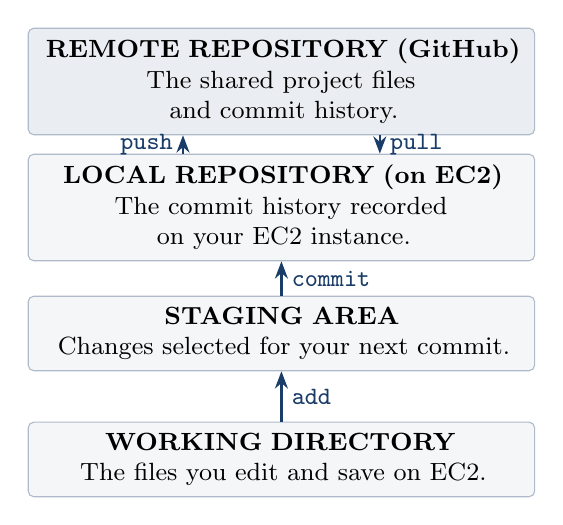
\begin{tikzpicture}[
        level/.style={draw=BootcampBlueDark!35,fill=SoftGray,
          rounded corners=2pt,text width=6.15cm,minimum height=0.82cm,
          align=center,font=\small,inner sep=4pt},
        flow/.style={-{Stealth[length=2.2mm]},thick,draw=BootcampBlueDark},
        action/.style={font=\small\ttfamily,text=BootcampBlueDark}
      ]
        \node[level,fill=BootcampBlueDark!9] (remote) at (0,4.8)
          {\textbf{REMOTE REPOSITORY (GitHub)}\\
           The shared project files and commit history.};
        \node[level] (local) at (0,3.2)
          {\textbf{LOCAL REPOSITORY (on EC2)}\\
           The commit history recorded on your EC2 instance.};
        \node[level] (stage) at (0,1.6)
          {\textbf{STAGING AREA}\\
           Changes selected for your next commit.};
        \node[level] (work) at (0,0)
          {\textbf{WORKING DIRECTORY}\\
           The files you edit and save on EC2.};
        \draw[flow] ([xshift=-1.25cm]local.north)
          -- node[left,action]{push} ([xshift=-1.25cm]remote.south);
        \draw[flow] ([xshift=1.25cm]remote.south)
          -- node[right,action]{pull} ([xshift=1.25cm]local.north);
        \draw[flow] (stage.north) -- node[right,action]{commit} (local.south);
        \draw[flow] (work.north) -- node[right,action]{add} (stage.south);
      \end{tikzpicture}
    \end{column}
    \begin{column}{0.41\textwidth}
      \textbf{Git records versions.}\par
      GitHub hosts a remote repository.
      \medskip
      \begin{block}{Where is ``local''?}
        In this course, Git runs on \textbf{AWS Linux EC2}.
        VS Code connects to EC2 so you can edit those files.
      \end{block}
      \smallskip
      \textbf{The repeated path}\par
      Save $\to$ add $\to$ commit $\to$ push.\par
      \medskip
      {\small Pull brings remote updates into your local repository
      and updates your working files.}
    \end{column}
  \end{columns}
\end{frame}

% SLIDE 2 -- 1.5 minutes. Use each student's own assignment URL.
\begin{frame}{Start in the right place}
  \begin{center}
    
\begin{tikzpicture}[
      box/.style={draw=BootcampBlueDark!30,fill=SoftGray,
        rounded corners=2pt,minimum height=1cm,align=center,
        font=\small,inner sep=5pt},
      flow/.style={-{Stealth[length=2mm]},thick,draw=BootcampBlueDark}
    ]
      \node[box,text width=2cm] (vscode) {\textbf{VS Code}\\on your laptop};
      \node[box,text width=2.4cm,right=0.75cm of vscode] (ec2)
        {\textbf{AWS Linux EC2}\\terminal + files};
      \node[box,text width=2.5cm,right=0.75cm of ec2] (repo)
        {\textbf{Local Git repo}\\inside EC2};
      \node[box,text width=2.45cm,right=0.75cm of repo] (github)
        {\textbf{GitHub}\\assignment repo};
      \draw[flow] (vscode) -- (ec2);
      \draw[flow] (ec2) -- (repo);
      \draw[flow] (repo) -- (github);
    \end{tikzpicture}
  \end{center}
  \smallskip
  \commandrow{git clone <url>}{Copies an existing remote repository and its history into a new local folder.}
  \commandrow{git status}{Shows which files are modified, staged, or untracked in the current repository.}
  \begin{block}{For your assignment}
    \small
    After accepting the Classroom 50 invitation, copy your own GitHub repository URL.
    Clone once into \texttt{\string~/FRE6883} on EC2. Open the cloned folder in VS Code;
    run the remaining commands inside that folder.
  \end{block}
  {\small Replace \texttt{<url>} with your URL, without brackets.
  Already cloned? Open the existing folder.}
\end{frame}

% SLIDE 3 -- 1.5 minutes. The staging area records the version at add time.
\begin{frame}{Save, select, record}
  \commandrow{git add <file>}{Stages the current saved changes in the named file for the next commit.}
  \commandrow{git add .}{Stages all non-ignored changes under the current folder, including additions and deletions.}
  \commandrow{git commit -m "message"}{Records the staged changes as a new local commit with a short description.}
  \begin{alertblock}{Two habits that prevent surprises}
    \textbf{Save before adding.} If you edit the file again, save it and add it again.\par
    \smallskip
    \textbf{Before \gitcmd{git add .}, check \gitcmd{git status}.}
    Make sure every listed file belongs in your commit.
  \end{alertblock}
  {\small A commit records the staged version; it stays on EC2 until you push.}
\end{frame}

% SLIDE 4 -- 1 minute. Keep integration mechanics outside this recitation.
\begin{frame}{Send your work; retrieve updates}
  \commandrow{git push}{Sends your local commits to the remote repository on GitHub.}
  \commandrow{git pull}{Retrieves remote updates and incorporates them into your local repository and working files.}
  \begin{columns}[T,onlytextwidth]
    \begin{column}{0.48\textwidth}
      \begin{block}{When starting work}
        Run \gitcmd{git status}, then \gitcmd{git pull} when your working directory is clean.\par
        \smallskip
        Have local edits? Save and commit your work first.
      \end{block}
    \end{column}
    \begin{column}{0.48\textwidth}
      \begin{block}{When sharing work}
        Save, add, commit, then \gitcmd{git push}.\par
        \smallskip
        Open your assignment repository on GitHub and verify the latest commit appears.
      \end{block}
    \end{column}
  \end{columns}
  \medskip
  {\small If Git stops with an error, read the message and ask for help.}
\end{frame}

% SLIDE 5 -- 1 minute. Distinguish saved unstaged edits from commit history.
\begin{frame}{Inspect before you act}
  \commandrow{git diff}{Shows saved, unstaged changes to files Git already tracks.}
  \commandrow{git log}{Shows the commit history leading to your current local version.}
  \begin{block}{Three different questions}
    \begin{tabularx}{\linewidth}{@{}l@{\hspace{1.2em}}X@{}}
      \gitcmd{git status} & Which files need attention? \\[0.4em]
      \gitcmd{git diff} & What lines have I changed since staging? \\[0.4em]
      \gitcmd{git log} & What work has already been committed?
    \end{tabularx}
  \end{block}
  \smallskip
  {\small \gitcmd{git diff} omits staged changes and new untracked files.
  Use \gitcmd{git status} to see their state.\par}
  \smallskip\par
  {\small If the output opens in a pager, press \texttt{q} to return to the terminal.}
\end{frame}

% SLIDE 6 -- 1.5 minutes. Ask for the sequence before revealing it.
\begin{frame}[t,fragile]{Scenario 1: get your code onto GitHub}
  You modified \texttt{Option01.cpp} and want your changes to appear on GitHub.
  \textbf{What commands should you run?}\par
  \smallskip
  {\small Assume you are in the correct EC2 repository and have saved the file.\par}
  \smallskip
  {\small\textbf{Think for 20 seconds; compare your sequence with a neighbor.}\par}
    \begin{uncoverenv}<2->
      \begin{exampleblock}{Expected sequence}
\begin{lstlisting}
git status
git add Option01.cpp
git commit -m "Implement CRR pricer"
git push
\end{lstlisting}
      \end{exampleblock}
      {\small After a successful push, refresh your GitHub repository to check the commit.}
    \end{uncoverenv}
\end{frame}

% SLIDE 7 -- 1 minute. Answer the command question while preserving local work.
\begin{frame}[t,fragile]{Scenario 2: the remote repository changed}
  You changed your local files. Your teammate or instructor has also updated
  the \textbf{same remote repository} on GitHub.
  \medskip\par
  \textbf{Which command retrieves those remote updates?}\par
  \smallskip
  {\small\textbf{Think for 15 seconds, then answer.}\par}
    \begin{uncoverenv}<2->
      \begin{exampleblock}{Answer}
\begin{lstlisting}
git pull
\end{lstlisting}
        First save your files, check \gitcmd{git status}, and add and commit your local work.
        Then pull the remote updates.
      \end{exampleblock}
      \smallskip
      {\small If Git cannot complete the operation, read its message and ask for help.}
    \end{uncoverenv}
\end{frame}

% SLIDE 8 -- 1 minute. Exercise inspection commands, not another upload sequence.
\begin{frame}[t,fragile]{Scenario 3: what changed, and what was recorded?}
  You saved edits to the tracked file \texttt{Option01.cpp}, but have not staged them.
  \medskip
  \begin{enumerate}
    \item Which command shows the changed lines?
    \item Which command shows earlier commits and their messages?
  \end{enumerate}
  \medskip
  {\small\textbf{Think for 15 seconds, then answer.}\par}
    \begin{uncoverenv}<2->
      \begin{exampleblock}{Answers, in order}
\begin{lstlisting}
git diff
git log
\end{lstlisting}
        \gitcmd{git diff} inspects your unstaged edits;
        \gitcmd{git log} inspects recorded commits.
      \end{exampleblock}
    \end{uncoverenv}
\end{frame}

% SLIDE 9 -- 1 minute. Five practical mistakes, each paired with a habit.
\begin{frame}{Common mistakes}
  \begin{itemize}
    \setlength{\itemsep}{1.0em}
    \item \textbf{Forgetting to save the file.}\\
      Save in VS Code before running \gitcmd{git add}.
    \item \textbf{Forgetting \gitcmd{git add}.}\\
      Stage the changes you want in the next commit.
    \item \textbf{Committing but forgetting to push.}\\
      Run \gitcmd{git push}, then verify the commit on GitHub.
    \item \textbf{Editing in the wrong folder or repository.}\\
      Check the EC2 connection, open folder, and terminal location.
    \item \textbf{Running commands blindly.}\\
      Read \gitcmd{git status} and Git's output before the next step.
  \end{itemize}
\end{frame}

% SLIDE 10 -- 1 minute. Screenshot reference: all commands on one static slide.
\begin{frame}{Git cheat sheet}
  \relax
  {\small\textbf{FRE6883:} VS Code $\to$ AWS Linux EC2 $\to$ local Git repository
  $\to$ GitHub / Classroom 50\par}
  \medskip
  {\small
    \renewcommand{\arraystretch}{1.0}
    \begin{tabularx}{\textwidth}{@{}l@{\hspace{2em}}X@{}}
      \toprule
      \textbf{Command} & \textbf{Purpose} \\
      \midrule
      \gitcmd{git clone <url>} & Copy a remote repository and its history locally; do this once. \\
      \gitcmd{git status} & Check modified, staged, and untracked files. \\
      \gitcmd{git add <file>} & Stage the saved changes in one file. \\
      \gitcmd{git add .} & Stage all non-ignored changes under the current folder. \\
      \gitcmd{git commit -m "message"} & Record the staged changes as a local commit. \\
      \gitcmd{git push} & Send local commits to GitHub. \\
      \gitcmd{git pull} & Retrieve remote updates and apply them locally. \\
      \gitcmd{git log} & Read the local commit history. \\
      \gitcmd{git diff} & Inspect saved, unstaged changes to tracked files. \\
      \bottomrule
    \end{tabularx}\par
  }
  \smallskip
  {\small
    \textbf{In your EC2 repo:} save $\to$ \gitcmd{git status} $\to$ add $\to$ commit $\to$ push
    $\to$ verify on GitHub.\par
    \textbf{To start:} check status; pull with a clean working directory. Save and commit local edits first.\par
  }
\end{frame}

\end{document}
